% Part: sets-functions-relations
% Chapter: arithmetization
% Section:reals

\documentclass[../../../include/open-logic-section]{subfiles}

\begin{document}

\olfileid[pt]{sfr}{arith}{real}
\olsection{A Reta Real}

O passo seguinte é mostrar como construir os reais a partir dos racionais.
Antes disso, há que perceber o que há de \emph{distintivo} nos reais.

Os reais comportam-se de modo muito parecido com os racionais. (Tecnicamente,
ambos são exemplos de \emph{corpos ordenados}; para a definição, ver
\olref[check]{orderedfield}.) Agora, se resolveu os exercícios de
\olref[sfr][siz][]{chap}, saberá que há estritamente mais reais do que racionais,
isto é, que $\cardless{\Rat}{\Real}$. Cantor foi o primeiro a provar isto. Há,
contudo, cerca de dois milênios e meio que se conhecem números irracionais, isto é,
reais que não são racionais. De fato:
%\footnote{Now: ``$\sqrt{2}$'' equally refers to both the positive and the negative roots; but in the next few pages, I'll forget about this, and consider only the positive root.}
\begin{thm}\ollabel{root2irrational}
$\sqrt{2}$ não é racional, isto é, $\sqrt{2} \notin \Rat$
\end{thm}

\begin{proof}
Suponhamos, por \emph{reductio}, que $\sqrt{2}$ é racional. Então $\sqrt{2} =
\nicefrac{m}{n}$ para alguns números naturais $m$ e $n$. De fato, podemos
escolher $m$ e $n$ de modo a que a fração não possa ser mais reduzida.
Reorganizando, $m^{2} = 2n^{2}$. A partir daqui, completamos a prova de duas
formas:

\emph{Primeiro, geometricamente} (seguindo Tennenbaum).\footnote{Esta prova é
relatada por \cite{Conway2006}.} Consideremos estes quadrados:
\begin{center}	
	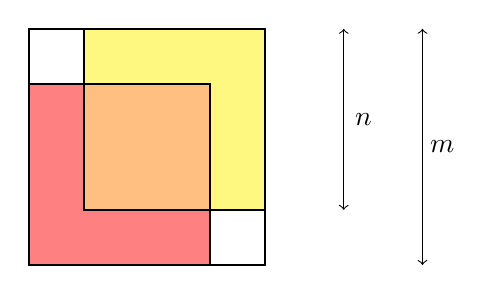
\begin{tikzpicture}
		\draw[thick] (0,0) rectangle (3,3);
		\draw[thick, fill=red!50] (0,0) rectangle (2.3,2.3);
		\draw[thick, fill=yellow!50] (0.7,0.7) rectangle (3, 3);
		\draw[thick, fill=orange!50] (0.7,0.7) rectangle (2.3, 2.3);
		\draw[<->] (4, 0.7)--(4, 3);
		\node at (4.25, 1.85) (n) {$n$};
		\draw[<->] (5, 0)--(5, 3);
		\node at (5.25, 1.5) (m) {$m$};
	\end{tikzpicture}
\end{center}
Como $m^2 = 2n^2$, a região em que os dois quadrados de lado $n$ se sobrepõem
tem a mesma área que a região que nenhum dos dois quadrados cobre; isto é, a área
do quadrado cor de laranja é igual à soma das áreas dos dois quadrados não
sombreados. Logo, se o quadrado cor de laranja tem lado $p$ e cada quadrado não
sombreado tem lado $q$, então $p^2 = 2q^2$. Mas então $\sqrt{2} = \nicefrac{p}{q}$,
com $p < m$, $q < n$ e $p, q \in \Nat$. Isto contradiz o fato de $m$ e $n$
terem sido escolhidos tão pequenos quanto possível.
		
\emph{Segundo, formalmente.} Como $m^{2} = 2n^{2}$, segue-se que $m$ é par. (É
fácil mostrar que, se $x$ é ímpar, então $x^2$ é ímpar.) Logo $m = 2r$, para
algum $r \in \Nat$. Rearranjando, $2r^2 = n^{2}$, 
		%				\begin{align*}
		%					(2q)^{2} &= 2n^{2}\\
		%					4q^{2} &= 2n^{2}\\
		%					2q^{2} &= n^{2}
		%				\end{align*}
logo $n$ também é par. Assim $m$ e $n$ são ambos pares, e portanto a fração
$\nicefrac{m}{n}$ \emph{pode} ser ainda reduzida. Contradição!
\end{proof}

De passagem, esta prova diagramática permite relembrar o material de
\olref[his][set][mythology]{sec}. Tennenbaum (1927--2006) era um matemático
inequivocamente moderno; mas a prova é inegavelmente bela, completamente rigorosa
e apela à intuição geométrica!

Em todo o caso: os reais são ``mais extensos'' do que os racionais. Nalgum
sentido, há ``lacunas'' nos racionais, e os reais preenchem-nas. Weierstrass
apercebeu-se de que isto descreve uma única propriedade dos números reais que os
distingue dos racionais, nomeadamente a \emph{propriedade de completude}:
\emph{Todo conjunto não vazio de números reais com majorante tem um supremo
(menor majorante).}

É fácil ver que os racionais não têm a propriedade de completude. Por exemplo,
considere-se o conjunto dos racionais menores que $\sqrt{2}$, isto é:
\[
	\Setabs{p \in \Rat}{p^2 < 2 \text{ ou }p < 0}
\]
Este conjunto tem um majorante nos racionais; os seus !!{element}s são todos
menores que $3$, por exemplo. Mas qual é o seu supremo? Queremos dizer
``$\sqrt{2}$''; contudo, acabamos de ver que $\sqrt{2}$ \emph{não} é racional. E
não existe racional mínimo entre os que são estritamente maiores que
$\sqrt{2}$. Logo, o conjunto tem majorante, mas não tem supremo. Assim, os
racionais não satisfazem a propriedade de completude.

Em contraste, o contínuo ``moralmente deveria'' ter a propriedade de completude.
Não queremos apenas que $\sqrt{2}$ seja um número real; queremos preencher todas
as ``lacunas'' da reta racional. Queremos, ainda, que o próprio contínuo não tenha
``lacunas''. É exatamente isso que obteremos via completude.

\end{document}
